\pdfoutput=1
% In particular, the hyperref package requires pdfLaTeX in order to break URLs across lines.

\documentclass[11pt]{article}

% Change "review" to "final" to generate the final (sometimes called camera-ready) version.
% Change to "preprint" to generate a non-anonymous version with page numbers.
\usepackage[preprint]{acl}

% Standard package includes
\usepackage{times}
\usepackage{latexsym}

% For proper rendering and hyphenation of words containing Latin characters (including in bib files)
\usepackage[T1]{fontenc}
% For Vietnamese characters
% \usepackage[T5]{fontenc}
% See https://www.latex-project.org/help/documentation/encguide.pdf for other character sets

% This assumes your files are encoded as UTF8
\usepackage[utf8]{inputenc}

% This is not strictly necessary, and may be commented out,
% but it will improve the layout of the manuscript,
% and will typically save some space.
\usepackage{microtype}

% This is also not strictly necessary, and may be commented out.
% However, it will improve the aesthetics of text in
% the typewriter font.
\usepackage{inconsolata}
\usepackage{amsmath}
\usepackage{amsfonts}
\usepackage{graphicx}
\usepackage{float}
\usepackage{tabularx} % For flexible-width columns
\usepackage{booktabs} % For nicer table rules
\usepackage{array}  % Extended col types if needed

% If the title and author information does not fit in the area allocated, uncomment the following
%
%\setlength\titlebox{<dim>}
%
% and set <dim> to something 5cm or larger.

\setlength{\parindent}{0pt} % No indentation
\setlength{\parskip}{0.2em} % Space between paragraphs
% Congfigure the table of contents and section numbering
\setcounter{tocdepth}{4}
\setcounter{secnumdepth}{4}

% \usepackage{microtype}
% \usepackage{inconsolata}
% \usepackage{amsmath}
% \usepackage{amsfonts}
% \usepackage{graphicx}
% \usepackage{float}
% \usepackage{tabularx} % For flexible-width columns
% \usepackage{booktabs} % For nicer table rules
% \usepackage{array}  % Extended col types if needed
% \usepackage{xspace} % add space after only if needed

% Configure \Cref to use \S for sections and \S\S for subsections
% \usepackage{hyperref} % must be loaded before cleveref
\usepackage{cleveref}
\usepackage[titletoc]{appendix}
\AtBeginEnvironment{appendices}{\crefalias{section}{appendix}}
\AtBeginEnvironment{appendices}{\crefalias{subsection}{appendix}}
\AtBeginEnvironment{appendices}{\crefalias{subsubsection}{appendix}}

% \crefnames{part,chapter,section}{\S}{\S\S}
% \crefnames{paragraph}{\P}{\P\P}
% \crefname{abstract}{abstract}{abstracts}

\newcommand{\numlist}[1]{(\textbf{#1})}

\newcounter{para}
\newcommand\numpara{\par\refstepcounter{para}{\thepara}.\space\textbf}


% need to add this to avoid "undefined control sequence" error in .bib
% Holmes paper
\newcommand{\recorder}{\textregistered}

% specific to this paper
\newcommand{\links}{\textbf{\textsc{Links}}}
\newcommand{\linksys}{\textbf{\textsc{LinkSYS}}}
\newcommand{\studentmodel}{Gemma-3-1b-it }
\newcommand{\teachermodel}{DeepSeek-R1 }
\newcommand{\judgemodel}{OpenAi's o3-mini }
\newcommand{\mnemonic}{$m$}
\newcommand{\vocabulary}{$v$}
\newcommand{\eg}{$e$}

\title{\textbf{LINKS}: Generate linguistically grounded mnemonic devices for English vocabulary learning with reasoning, multilingual LLMs
}

\author{%
  My (Chiffon) Nguyen \\
  College of Computational Sciences \\
  Minerva University \\
  chiffonng@uni.minerva.edu
}

\begin{document}
\begin{titlepage}
\centering
{\scshape\LARGE Minerva University \par}
\vspace{1cm}
\begin{center}
  
\includegraphics[width=0.4\linewidth]{minerva/minerva_logo.pdf}
\end{center}
{\scshape\Large Capstone: Class of 2025 \par}
\vspace{1.5cm}
{\huge\bfseries LINKS: Generate linguistically grounded mnemonic devices for English vocabulary learning with reasoning, multilingual LLMs \par}
\vspace{2cm}
{\scshape\large Tra My (Chiffon) Nguyen \par}

\vfill
submitted in partial fulfillment of the requirements for the degree of \\ Bachelor of Science in Computational Sciences \par
\vspace{2cm}
{\large Capstone Committee \par}
Dr. Patrick Watson \\
Dr. Philip Sterne \\
\vspace{2cm}
{\large \today\par}
\end{titlepage}

\onecolumn
\section*{Executive Summary} \label{sec:exec-summary}
%% TODO: Explain the project to a non-technical audience.
% - What is the problem?
% - What is the solution?
% - What is the impact?
% - What is the next step?

Tags: computational linguistics, natural language processing, large language model, language education, english as a foreign language, vocabulary acquisition, synthetic data generation.

\subsection*{AI Statement} \label{sec:ai-statement}

The main idea of this project is to use large language models (LLMs) to generate mnemonic devices for English vocabulary learning. Such AI usage is documented in the main paper.

I extensively used Claude 3.7 Sonnet connected with my codebase to \numlist{1} generate working Python code for major features and plots, \numlist{2} debug my code and \numlist{3} iteratively improve my codebase with best practices including refactoring, modularization, and documentation. I also used Claude to aid producing this paper by \numlist{4} generating LaTex figures and tables, such as \Cref{fig:good-bad-mnemonics} and \Cref{tab:significance-llm-judge}, \numlist{5} explaining new methods used, especially GRPO (\Cref{app:grpo}), and \numlist{6} rewriting some sections of the paper to improve clarity and conciseness, particularly Abstract and \Cref{sec:discussion}.

There were several instances where AI failed to help, mostly due to \numlist{1} the usage of AI-related knowledge and packages that are recently released or updated, such as \verb|trl|'s \verb|GRPOTrainer| class, or and \numlist{2} low-frequency knowledge, such as some TeX formatting or lower-level software or hardware issues. An example: I failed to send API requests to \teachermodel from \verb|curator| but not from \verb|openai| library, due to SSL certificate issue. The root cause was a conflict between different Python versions installed globally on my laptop, one from \verb|homebrew| and one from Python distribution.

\subsection*{Important Notes} \label{sec:important-notes}

Due to limited compute, some experiments conducted are small-scale and need more data for robust validation and conclusion. However, the codebase is reproducible and scalable when there is more compute. All links, including this paper source .tex, is included on \hyperlink{https://github.com/chiffonng/mnemonic-gen}{Github}.

This project went through multiple technical iterations behind the scene, from supervised finetuning (Nov 2024) to group releative policy optimization (Feb 2025) (for details refer to \Cref{app:previous-iterations}). The main paper only discussed the final iteration, which is the most promising one. The other iterations are not included in the paper but their implementation is available in the codebase in forms of Jupyter Notebooks and old pull requests.

\clearpage

\tableofcontents


\maketitle
\begin{abstract}
To acquire advanced vocabulary, English learners often use mnemonic devices, memorable associations linking a new concept to learned concepts to improve memory and recall. Reviewing the literature on mnemonic techniques, we characterize good mnemonics as \textbf{linguistically grounded}, which better link to the target vocabulary, improving long-term retention and linguistic knowledge, especially at advanced levels (CEFR B2+). We investigate whether Large Language Models can consistently help write such effective mnemonics, with three different settings: in-context learning, and reasoning distillation. Concretely, we first measured different prompting strategies with a frontier reasoning model, \teachermodel, and generated \links, a synthetic dataset of 2000 triplets of \textit{reasoning trace, mnemonic, and example sentence} for 2000 vocabulary useful for TOEFL iBT \footnote{Internet-based Test of English as a Foreign Language}, IELTS Academic \footnote{International English Language Testing System}, and SAT\footnote{Scholastic Aptitude Test}. Second, using a subset of \links, we distilled linguistic reasoning from the \textit{teacher model} to the \textit{student model}, \studentmodel\footnote{\url{https://huggingface.co/collections/google/gemma-3-release-67c6c6f89c4f76621268bb6d}} , with online reinforcement learning. The trained, quantized model can be served with a local application such as OpenWebUI (interface) and Ollama (command-line).

Preliminary evaluation shows

The project examplifies that carefully designed NLP systems can generate resources for language learning, either in classroom settings or in self-study. Code, models, and dataset are available\footnote{Links: \url{https://github.com/chiffonng/mnemonic-gen}}.
\end{abstract}


\section{Introduction}
Vocabulary acquisition challenges many English language learners, particularly at upper intermediate to advanced levels where abstract and academic vocabulary predominates. Mnemonics, cognitive tools that help learners create associations between new vocabulary and familiar concepts, serve as valuable tools for enhancing retention and recall. The deeper learners elaborate the connection between the mnemonic and the target vocabulary, the longer and better they can recall the term. However, creating such effective mnemonics demands both linguistic expertise and creative effort, presenting a significant barrier for most learners. Large Language Models (LLMs) have demonstrated capabilities as knowledge bases and creative text generators, suggesting their potential for automated mnemonic generation.

Previous work explored automated mnemonic generation through computational methods using the \textbf{keyword method}, which involves 1) generateing simpler keywords that together sound or look like the target vocabulary and 2) creating memorable explanations that include the vocabulary, the keywords, amd its meaning \citep{atkinsonApplicationMnemonicKeyword1975}. \citet{savvaTransPhonerAutomatedMnemonic2014} and \citet{OzbalAUTOMATION2014} generated keywords of phonetic and orthographic similarities in the native language for foreign language vocabulary, across multiple languages. \citet{LeeSMARTPHONE2023} extended this work and utilized LLMs to produce phonetically similar keywords and visual cues and \citet{LeeEXPLORING2024} prompted LLMs to generate multiple mnemonic candidates and evaluate them based on imageability and coherence. Most recently, \citet{balepurSMART2024} fine-tuned LLaMA-2-70B on 800 crowd-sourced mnemonics and aligned outputs with learner preferences and learning outcomes.

%%%% Figure Highlight the difference between keyword "mnemonic" and "linguistically grounded mnemonics" with an example
%%% (e.g., \textbf{preposterous} can be broken down as pre- (before) + poster (after) + ous. Anything that comes both before and after is preposterous)

Although the keyword method is commonly used and empirically validated in classroom and laboratory contexts \citetext{\citealp{atkinsonApplicationMnemonicKeyword1975}, \citealp{pressleyMnemonicKeywordMethod1982}}, it may lead to longer retrieval time \citep{vanhellKeywordMnemonicsRote1997} and be inadequate for fairly abstract vocabulary \citetext{\citealp{camposLimitationsMnemonicKeywordMethod2003}, \citealp{camposImportanceKeywordGenerationMethod2004a}}. Such methods typically neglect other rich linguistic knowledge embedded in LLMs that could provide diverse mnemonic strategies beyond simple keyword associations. Second, previous works passively deliver generated mnemonics to learners. While \textsc{Smart} \citep{balepurSMART2024} was further trained on learners' preferences, these preferences were aggregated, potentially missing alignment with individual learning styles. Language learners who use self-created mnemonics retain vocabulary more effectively and for longer duration \citep{madanExploringWordMemorability2021}.

Our contributions can be summarized as follows. (\textbf{1}) We demonstrate that LLMs can generate \textbf{linguistically grounded mnemonics}, which emphasizes the importance of linguistic features in creating effective mnemonics, through reasoning and creative writing. (\textbf{2}) We present \links, a synthetic dataset of 2000 triplets of \textit{reasoning trace, mnemonic, and example sentence} for 2000 vocabulary. They can be integrated in a spaced repetition system (SRS) or language learning applications for vocabulary acquisition with better retrieval. (\textbf{3}) We distill the reasoning capabilities of a frontier, reasoning LLM, into a smaller model, \studentmodel, using \citep{DeepSeek-AIDEEPSEEKR12025}. The trained model \links, can be served locally, enabling users to generate mnemonics without relying on external APIs or internet connectivity.

\section{Background} \label{sec:background}

We assume a background on LLMs, including their transformer-based architecture (\Cref{app:llm-transformer}), in-context learning (\Cref{sec:icl-performance}), and reinforcement learning (full preliminaries are provided in \Cref{app:technicality}). We briefly review the literature on mnemonic devices for vocabulary learning and the use of LLMs in linguistic tasks.

\subsection{Mnemonic devices for vocabulary learning} \label{sec:mnemonic-review}

% TODO: Add a figure for what good mnemonics means. Here is a placeholder
% \begin{figure*}[htb]
%   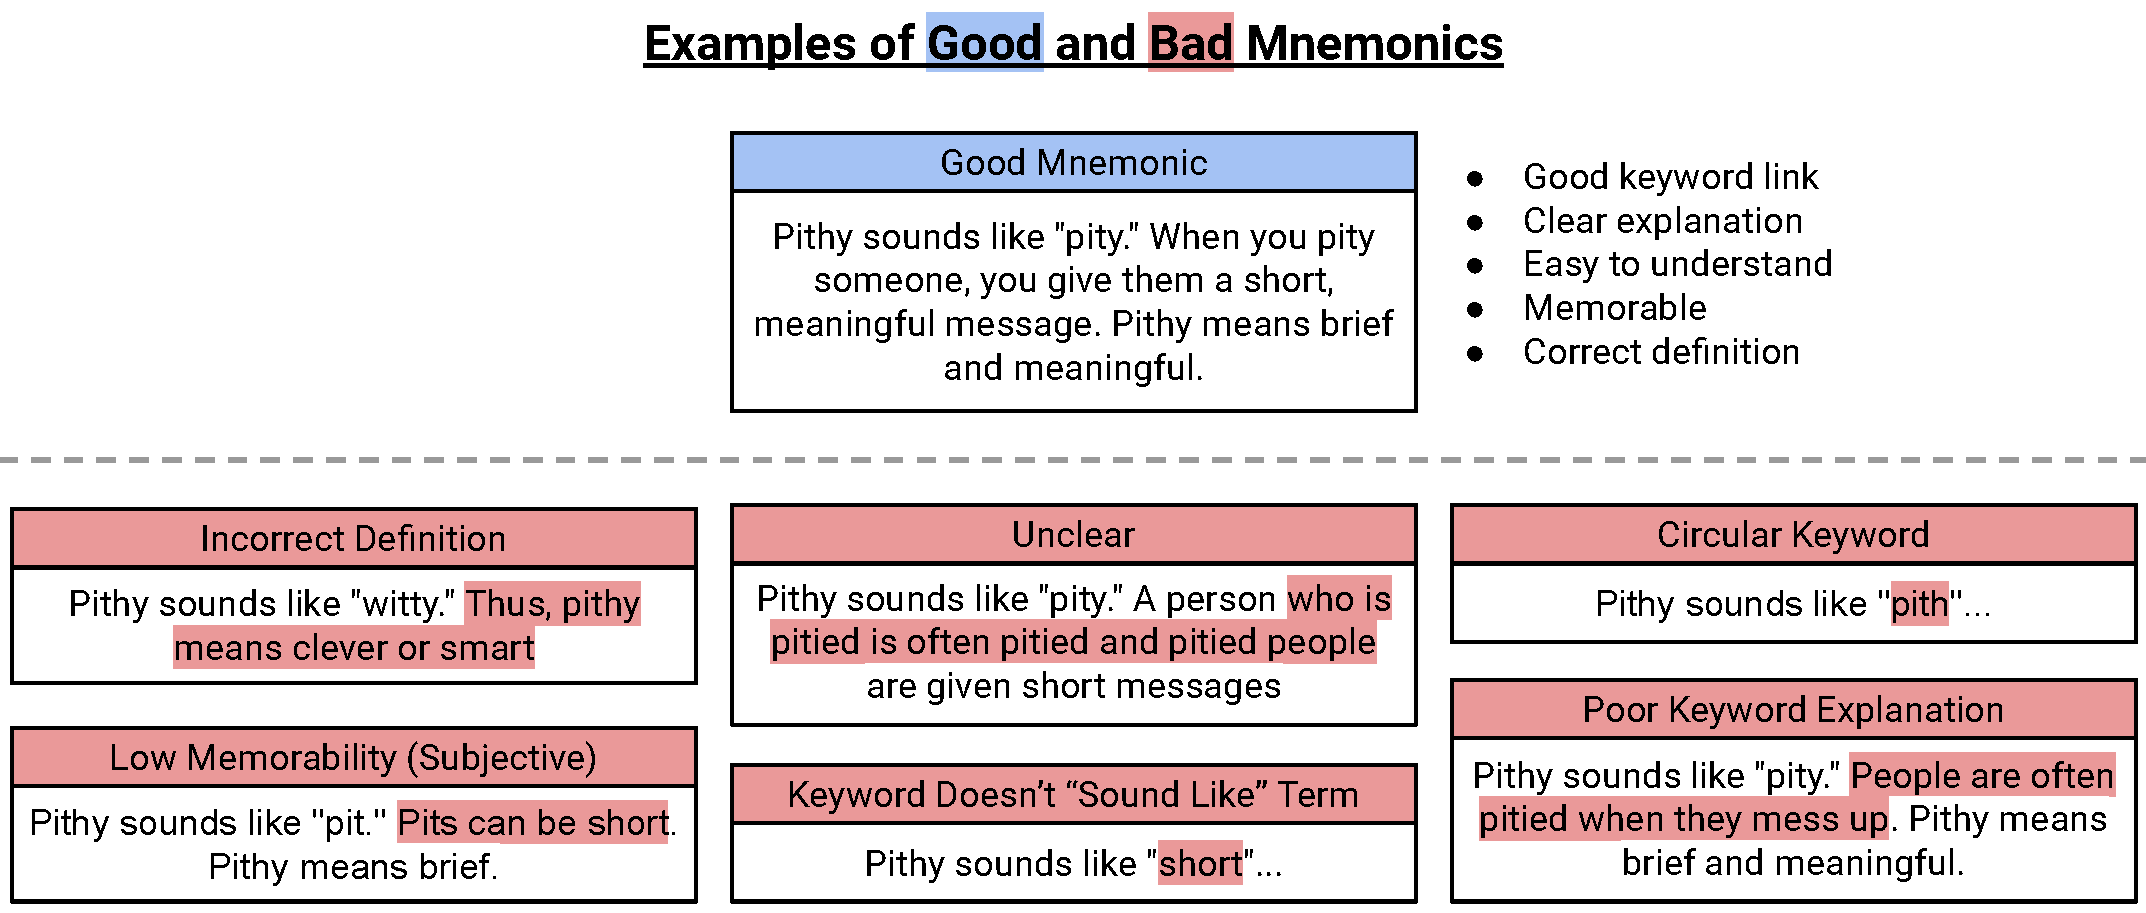
\includegraphics[width=\linewidth]{figures/good_bad_mnemonics.pdf}
%   \caption{Non-exhausitive list of characteristics of a good mnemonic, inferred from \citetext{\citealp{BalepurSMART2024}; \citealp{CamposUSING2011}; \citealp{luExplorationMnemonicsESL2015}; \citealp{SariogluUSE2024}}.}
%   \label{fig:good-bad-mnemonics}
% \end{figure*}

% Define custom colors


% Define custom box styles
\tcbset{
    goodbox/.style={
        colback=goodlight,
        colframe=goodgreen,
        fonttitle=\bfseries\color{white},
        coltitle=white,
        colbacktitle=goodgreen,
        enhanced,
        attach boxed title to top center={yshift=-1mm},
        boxed title style={sharp corners},
        top=2mm,
    },
    badbox/.style={
        colback=badlight,
        colframe=badred,
        fonttitle=\bfseries\color{white},
        coltitle=white,
        colbacktitle=badred,
        enhanced,
        attach boxed title to top center={yshift=-1mm},
        boxed title style={sharp corners},
        top=2mm,
    }
}

% Start the figure environment
\begin{figure*}[htb]
\centering
\footnotesize
% First row - Good mnemonic + characteristics
\begin{minipage}{0.66\textwidth}
    \begin{tcolorbox}[goodbox, title=Good Mnemonic]
        \textcolor{red}{\textbf{preposterous}}: \textcolor{goodgreen}{comes from pre- ("before") + post ("after") + -ous}, meaning reversed or absurd. \textcolor{orange}{An event cannot happen both pre- (before) and post- (after) to us, it is prespoterous!}
    \end{tcolorbox}
\end{minipage}
\hspace{0.5em}
\begin{minipage}{0.3\textwidth}
    \begin{itemize}[leftmargin=*, nosep]
        \item \vocab is used correctly in \mnem
        \item Clear \assoc linking \vocab and \mnem
        \item Strong \assoc
        \item \mnem uses similar or lower vocabulary than \vocab
        \item \mnem is memorable
    \end{itemize}
\end{minipage}

\vspace{0.3cm}

% Second row - 3 bad mnemonics
\begin{minipage}{0.33\textwidth}
    \begin{tcolorbox}[badbox, title=Incorrect Definition]
        Preposterous means very important or significant.
    \end{tcolorbox}
\end{minipage}%
\begin{minipage}{0.33\textwidth}
    \begin{tcolorbox}[badbox, title=Circular Association]
        Preposterous sounds like preposterous.
    \end{tcolorbox}
\end{minipage}%
\begin{minipage}{0.33\textwidth}
    \begin{tcolorbox}[badbox, title=Weak Association]
        Preposterous sounds like prosperous. Preposterous people usually make prosperous business decisions.
    \end{tcolorbox}
\end{minipage}

\vspace{0.3cm}

% Third row - 3 more bad mnemonics
\begin{minipage}{0.33\textwidth}
    \begin{tcolorbox}[badbox, title=Difficult Vocabulary]
        Preposterous means ludicrously implausible or contrary to conventional hierarchies of logical induction.
    \end{tcolorbox}
\end{minipage}%
\begin{minipage}{0.33\textwidth}
    \begin{tcolorbox}[badbox, title=Too Abstract]
        Preposterous describes logical fallacies where the premise negates itself through temporal displacement.
    \end{tcolorbox}
\end{minipage}%
\begin{minipage}{0.33\textwidth}
    \begin{tcolorbox}[badbox, title=Offensive Content]
        Preposterous contains "post" which reminds me of [inappropriate culturally-specific reference].
    \end{tcolorbox}
\end{minipage}

\caption{Characteristics of good mnemonics, and examples of bad mnemonics. We propose VAM/VEM model, where a good mnemonic must have three components: \vocabulary (\vocab), \association (\assoc) (or explanation ($e$)), and \mnemonic (\mnem), with characteristics listed above. These characteristics are also available in list (\Cref{app:mnemonic-characteristics})}
\label{fig:good-bad-mnemonics}
\end{figure*}


Mnemonic devices are mental techniques that enhance memory through meaningful associations between new information and pre-existing knowledge \citep{pressleyMnemonicKeywordMethod1982,PintrichROLE2002}. For vocabulary acquisition, the keyword method has been widely studied. The method involves creating acoustically or orthographically similar keywords to the target vocabulary, followed by an association between these keywords and the word's meaning \citep{atkinsonApplicationMnemonicKeyword1975}.

While the keyword method has shown effectiveness in classroom and laboratory contexts, its success often relies on several factors. It enhances recall for concrete vocabulary, since learners can easily create mental imagery for it \citep{schwanenflugelContextAvailabilityRecall1992,wangKeywordMnemonicRetention1992}. However, its effectiveness diminishes for abstract vocabulary \citep{fothMnemonicTechniqueEffectiveness1973,CamposLIMITATIONS2003},  experienced language learners with high proficiency \citep{vanhellKeywordMnemonicsRote1997,CamposUSING2011}, and mnemonics not created by the learners themselves \citep{camposImportanceKeywordGenerationMethod2004a,madanExploringWordMemorability2021}, sometimes with longer recall and lower retention than rote learning.

More linguistically sophisticated approaches, such as etymology-based mnemonics, could provide deeper encoding and potentially stronger retention for abstract vocabulary \citep{ piersonUsingEtymologyClassroom1989,akarslanEffectsTeachingWord2019, gangavarapuUsingEtymologyVocabulary2024}. These approaches leverage morphological, etymological, and semantic properties of words, creating more meaningful associations that align with how language is naturally structured \citep{zhangApplicationEtymologySemantic2013}.

Psycholinguistics offers other insights into factors that enhance mnemonic recall by investigating memorability, how easily information is remembered, based on its inherent characteristics and the context in which it appears. Mnemonics are more effective when they incorporate animate entities, indicators of potential usefulness, and concrete visual imagery \citep{schwanenflugelContextAvailabilityRecall1992,ledingAdaptiveMemoryAnimacy2019,madanExploringWordMemorability2021}. Moreover, emotionally charged associations produce stronger memory traces than neutral ones \citep{altarribaConcretenessContextAvailability1999}, and mnemonics that involve deeper linguistic analysis yield more robust recall \citep{rankinAgePresentationRate1983, SariogluUSE2024}. These findings underscore the importance of both the content and the cognitive strategies applied during encoding in achieving optimal memorability.

We explore these principles in our work, focusing on how LLMs can generate mnemonics that incorporate good characteristics (\Cref{fig:good-bad-mnemonics}) and leverage linguistic features (\Cref{tab:linguistic-features}).

\subsection{LLMs: linguistic competence, reasoning, and creativity} \label{sec:llm-linguistic-competence}

Significant advancements have been made in enhancing the reasoning capabilities of large language models (LLMs), particularly in mathematical and scientific domains where problems have unique correct answers. Several prompting techniques were introduced to make LLMs learn from demonstrations (or "shots") or produce explicit step-by-step thinking processes to improve their reasoning, notably few-shot prompting \citep{brownFewShotLearners2020}, chain-of-thought (CoT) \citep{weiChainofThoughtPromptingElicits2022}, self-consistency \citep{wangSelfConsistencyImprovesChain2022}, zero-shot reasoning \citep{kojimaZeroShotReasoners2022}, analogical reasoning (automated few-shot CoT) \citep{YasunagaLLMAnalogicalReasoners2023}. Post-training techniques such as reinforcement learning from human feedback (RLHF) \citep{ouyangRLHF2022} and CoT data \citep{DeepSeek-AIDEEPSEEKR12025} further endows LLMs with instruction-following and reasoning capabilities. However, LLMs still struggle with complex reasoning tasks that require multiple steps, abstract thinking \citep{weiChainofThoughtPromptingElicits2022} or low-frequency knowledge \citep{kandpalLongTailKnowledge2023,sunHeadtoTailHowKnowledgeable2024}.

The ability to use and reason through languages falls into the categories of long-tail knowledge and abstract reasoning. Recent studies have explored LLMs' linguistic competence, defined as their ability to understand and apply language rules and patterns \citep{waldisHOLMES2024}. LLMs typically perform better on formal linguistic competence tasks, such as morphology and syntax, than on functional linguistic competence tasks, such as semantics, discourse \citep{KhoujaLINGOLYTOO2025} or phonology \citep{suvarnaPhonologyBenchEvaluatingPhonological2024}. Their competence is influenced by model architecture, with encoder-based models often outperforming decoder-only models, and larger models generally showing better linguistic understanding \citep{waldisHOLMES2024}. Instruction tuning could improve performance on linguistic tasks, though sometimes at the expense of deeper language understanding \citep{waldisHOLMES2024,yinDidYouRead2023}.

LLMs can also perform inductive multilingual reasoning, primarily demonstrated through inferring rules in linguistic puzzles as seen in International Olympiad in Linguistics, especially when provided with analogical demonstrations \citep{RamjiINDUCTIVE2024}. However, its reasoning remains inconsistent, with performance varying across minor problem perturbations, suggesting that it may not fully understand the underlying linguistic principles and memorize it \citep{RamjiINDUCTIVE2024,KhoujaLINGOLYTOO2025}. This inconsistency is also observed in mathematical reasoning tasks, where LLMs can produce correct answers but often fail to provide coherent explanations \citep{weiChainofThoughtPromptingElicits2022}.

For mnemonic generation specifically, previous work has explored using LLMs for automated keyword mnemonic generation \citep{LeeSMARTPHONE2023, LeeEXPLORING2024, BalepurSMART2024}, but these approaches have primarily focused on phonetic similarity rather than leveraging the broader linguistic knowledge embedded in LLMs. Our work extends these efforts by exploring how LLMs can use linguistic reasoning abilities to incorporate multiple linguistic features to generate mnemonic devices.




\section{In-context learning performance} \label{sec:icl-performance}

%% TODO: Review in-context learning literature here, including CoT, few-shot prompting, and zero-shot prompting. Discuss the differences between these methods and their implications for LLMs' performance in generating mnemonics.
\subsection{Experimental setup}
We systematically compared various in-context learning approaches to understand how different prompting techniques affect mnemonic generation. \Cref{fig:prompting-methods} illustrates the percentage of linguistically grounded mnemonics generated by different prompt formulations.

We used \verb|curator| \citep{BespokeLabBESPOKE2025} with \verb|litellm| orchestration layer to interact with LLM APIs, simpify API calls, manage rate limits, and handle retries.

\subsection{Results}

\begin{figure}
  \centering
  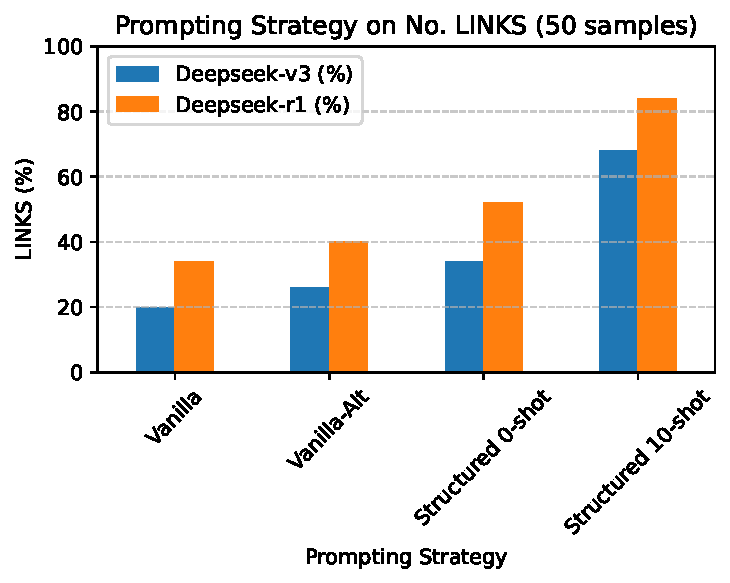
\includegraphics[width=\linewidth]{figures/prompt_comparison.pdf}
  \caption{Comparison of prompting methods (see detailed prompt in \Cref{app:prompt-usage}). Y-axis shows percentages of linguistically-grounded mnemonics generated out of 50 requests sent for each prompt type.}
  \label{fig:prompting-methods}
\end{figure}

We observed significant variation in the quality and linguistic grounding of generated mnemonics based solely on prompt formulation. Four distinct prompting strategies were evaluated (see details in \cref{app:prompt-usage})
Vanilla
Reasoning LLMs tend to overthink \citep{xuChainDraftThinking2025}
Good practices: provide decomposed instructions, structured output format, demonstration examples \citep{MishraREFRAMING2022}, and clarify definitions of linguistic features \citep{yinDidYouRead2023}

compress task definition \citep{yinDidYouRead2023},


\section{Knowledge and reasoning distillation} \label{sec:distillation}

\begin{figure}[htb]
  \centering
  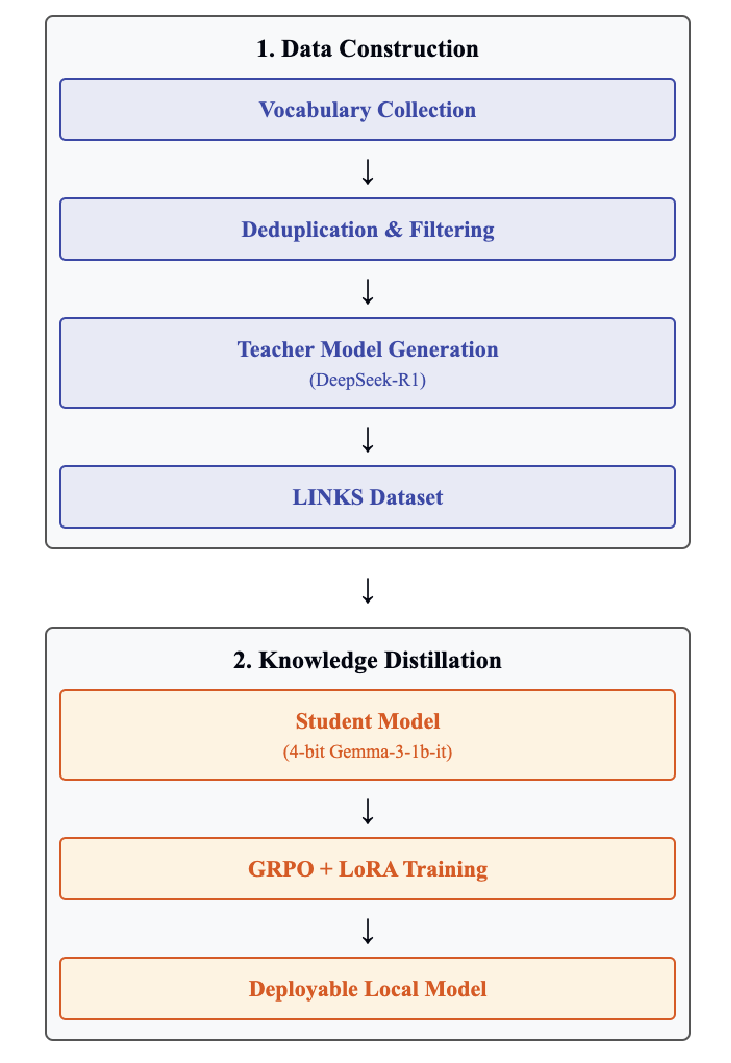
\includegraphics[width=\linewidth]{figures/pipeline.pdf}
  \caption{\linksys pipeline. The pipeline consists of two main components: (1) CoT data generation and (2) model distillation. We generate a dataset of mnemonics with reasoning traces using a large language model (LLM) as a teacher. Then we distill the reasoning capabilities of the teacher model into a smaller student model using GRPO \Cref{app:grpo}. Finally, we obtain \linksys, a smaller model that can generate mnemonics through linguistic reasoning.}
  \label{fig:distillation}
\end{figure}

\subsection{Preparation} \label{sec:data-prep}
We first created a comprehensive training dataset. Following best practices in synthetic data generation with LLMs \citetext{\citealp{longLLMsDrivenSyntheticData2024b}, \citealp{openthoughtsteamOpenThoughts2025}}, we designed a data construction pipeline with key components (\Cref{fig:distillation}).

\paragraph*{Vocabulary selection} \label{sec:vocab-selection}
We collected 5,000 distinct words from three main sources: English as a foreign language tests (TOEFL iBT, IELTS Academic), standardized tests with verbal reasoning (SAT, GRE), and CEFR C1/C2 word lists. This ensured coverage of academic and abstract vocabulary that would benefit from mnemonic devices. After fuzzy-matching deduplication (threshold 95\%), we refined the dataset and performed stratified random sampling (stratified by linguistic features used) to obtain 2,000 distinct vocabulary for post-training.

\paragraph*{Prompt design and model selection} Based on \cref{sec:icl-performance}'s findings, we designed system and user prompts, focusing on the 10-shot CoT approach that demonstrated superior performance in eliciting linguistic reasoning and creating memorable, \lgms.

\subsection{Dataset generation} \label{sec:data-gen}

Using our optimized prompts and vocabulary list, we generated the \links dataset of approximately 2,000 entries, each containing:

\begin{equation}
(\tau_i, m_i, e_i) \in \mathcal{D}
\end{equation}

where $\tau_i$ represents the reasoning trace exploring linguistic features, $m_i$ the generated mnemonic, and $e_i$ an example sentence for vocabulary $i$. The dataset creation process can be formalized as:

\begin{equation}
(\tau_i, m_i, e_i) = f_{\text{teacher}}(v_i; p_{\text{CoT}})
\end{equation}

where $f_{\text{teacher}}$ is the teacher model function, $v_i$ is vocabulary $i$, and $p_{\text{CoT}}$ is our 10-shot CoT prompt.

\subsection{Quality control} To ensure the quality of the generated mnemonics, we implemented a multi-step validation process. We first filtered out any entries that did not meet our structured output format or contained incomplete reasoning traces. We then performed a manual review of a random sample of 200 entries to assess the linguistic grounding and coherence of the mnemonics. This review process involved checking for clear connections between the vocabulary and the mnemonic, as well as ensuring that the example sentence accurately reflected the vocabulary's meaning.

\subsection{Training and inference} \label{sec:training-inference}
To transfer the linguistic reasoning capability to a smaller model, we implemented a distillation process using Group Relative Policy Optimization (GRPO).

We selected Google's \studentmodel \citep{gemma-teamGemma3Technical2025} as our student model due to its balance of performance and size (1 billion parameters). It can handle general-purpose tasks in multiple languages, and demonstrate instruction-following abilities. We used a 4-bit quantized version to further reduce memory requirements while maintaining performance \citep{dettmersQLoRAEfficientFinetuning2023}.

\paragraph*{Group Relative Policy Optimization (GRPO)} We employed GRPO \citep{DeepSeek-AIDEEPSEEKR12025} to distill the reasoning capabilities into the student model. For each input prompt $q$ generating a vocabulary $v$, the model produces $G$ candidate outputs:

\begin{equation}
O_q = \{o_1, o_2, \ldots, o_G\}
\end{equation}

These outputs are evaluated using reward functions $r_j$ that output scores, with the overall reward for output $i$ calculated as:

\begin{equation}
r_i = \sum_{j=1}^{J} w_j r_j(o_i, v)
\end{equation}

where $w_j$ is the weight for reward function $j$. We provide more technical details in \Cref{app:grpo}, including the policy loss to be minimized.

We defined three reward functions $r$ that encode essential characteristics of effective mnemonics:
\numlist{1} adherence to the structured format with reasoning, mnemonic, and example,
\numlist{2} usage of the target vocabulary in the mnemonic, penalizing bad mnemonics such as acronyms, and
\numlist{3} explicit incorporation of linguistic features in \Cref{tab:linguistic-features} or a reasonable custom feature.

We assigned higher weights to criterion 3, and generated $G=2$ candidates per training example to enable learning from comparisons. Training was performed on a single NVIDIA H100 GPU for approximately 4 hours (more details in \Cref{app:grpo-config}).

\paragraph*{Low-Rank Adaptation (LoRA)} We trained \studentmodel using GRPO wrapped in LoRA layers (\Cref{app:lora-config}) to reduce the number of trainable parameters and rank-stabilized LoRA that maintains stability for adapters with higher ranks.

\section{Evaluation} \label{sec:evaluation}
We evaluated the performance of \linksys in two main ways: \numlist{1} qualitative grading with LLM-as-a-judge and \numlist{2} pairwise preference using double-blind annotations. The first method involved using another LLM, \judgemodel, to evaluate the quality of mnemonics generated by our model, while the second involved annotators comparing mnemonics generated by the base model, \studentmodel, and our model, \linksys.

\begin{table*}[!htb]
\centering
\caption{Metric comaparison between the base (\studentmodel) and \linksys models}
\label{tab:significance-llm-judge}
\begin{tabular}{lccccc}
\toprule
\textbf{Evaluation Metric} & \textbf{Base} ($\mu$) & \linksys ($\mu$) & $\mu$ diff. & \textbf{p-value} & \textbf{Effect size} \\
\midrule
Correct vocabulary usage (bool) & 0.755 & 0.795 & +0.040 & 0.077 & -- \\
Linguistic grounding (bool) & 0.670 & 0.735 & +0.065 & \textbf{0.009} & -- \\
Association strength (1-5) & 2.845 & 3.070 & +0.225 & \textbf{<0.001} & 0.464 \\
Clarity (1-5) & 3.155 & 3.410 & +0.255 & \textbf{<0.001} & 0.481 \\
Memorability (1-5) & 2.600 & 2.900 & +0.300 & \textbf{<0.001} & 0.566 \\
\bottomrule
\end{tabular}
\begin{minipage}{\textwidth}
\vspace{0.1em}
\small
\textit{Note:} Bold p-values indicate statistically significant differences ($p < 0.05$). Effect sizes are Cohen's d, where 0.2 is small, 0.5 is medium, and 0.8 is large. Boolean metrics (first two rows) do not have effect sizes.
\end{minipage}
\end{table*}


\subsection{Qualitative grading with LLM judge} \label{sec:qualitative-llm-judge}

We designed a structured evaluation protocol using \judgemodel as a judge to assess mnemonic quality. The LLM judge evaluated 200 pairs of mnemonics from our test set, with each pair generated by the base model (\studentmodel) and our model \linksys.

We asked the judge to score each mnemonic independently on four metrics from our VAM model (\Cref{fig:good-bad-mnemonics}):
\numlist{1} whether the vocabulary is used correctly in the mnemonic,
\numlist{2} strength of association between the vocabulary and the mnemonic,
\numlist{3} how clear and easy to understand the mnemonic is,
\numlist{4} how memorable the mnemonic is, considering factors like concreteness, imageability, and distinctiveness. The last metric is \numlist{5} whether the mnemonic is linguistically grounded, meaning it incorporates linguistic features such as phonetics, morphology, or etymology.

Each criterion was evaluated on a binary scale (correct usage, linguistic grounding) or a 5-point Likert scale (association, clarity, memorability). The judge was instructed to provide six-field output: the score for each metric, and a brief reasoning for those scores.

We also calculated whether the difference in ratings was statistically significant using \numlist{1} a Wilconoxon signed-rank test for Likert ratings with paired samples and \numlist{2} a McNemar's test for paired boolean ratings. We set the significance level at 0.05.

\begin{figure}[htb]
  \centering
  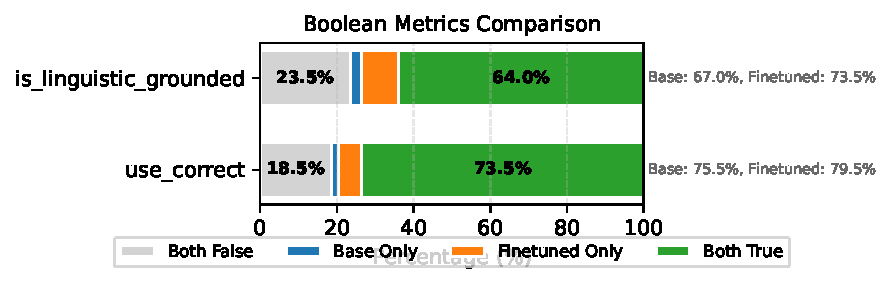
\includegraphics[width=\linewidth]{figures/boolean_comparison.pdf}
  \caption{LLM-as-a-judge evaluation for boolean metrics (true/false): correct usage of vocabulary in mnemonic and linguistic grounding of mnemonic. \linksys shows improvement in both metrics, with notable gains in linguistic grounding (68\% vs. 82\%).}
  \label{fig:llm-judge-boolean}
\end{figure}

\begin{figure}[htb]
  \centering
  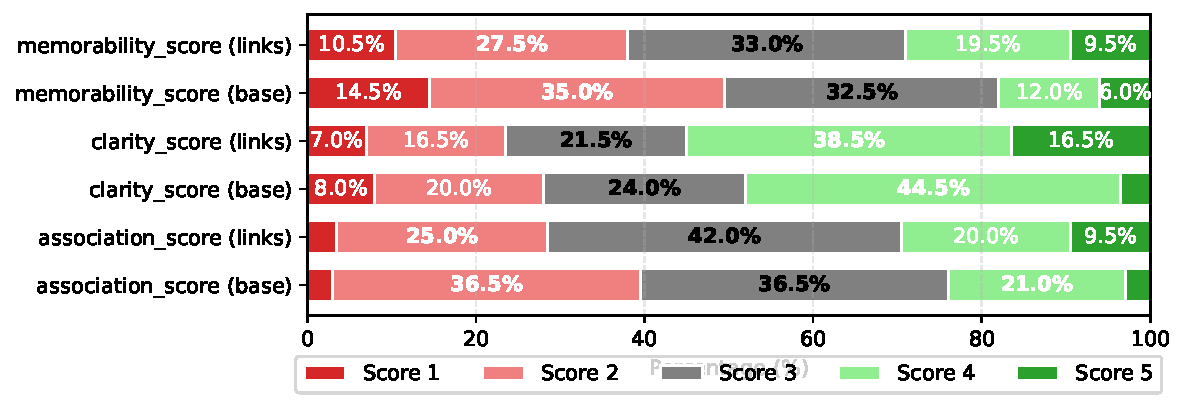
\includegraphics[width=\linewidth]{figures/likert_distribution.pdf}
  \caption{LLM-as-a-judge evaluation for 5-point Likert scale metrics. \linksys shows improvements across all three metrics, with the most significant gains in memorability (mean of 2.6 vs. 2.9)}
  \label{fig:llm-judge-likert}
\end{figure}

We reported the distribution of \judgemodel's ratings in \Cref{fig:llm-judge-boolean,fig:llm-judge-likert}, and summarized the difference in performance between the base model (\studentmodel) and our model in \Cref{tab:significance-llm-judge}. The results indicate that \linksys outperforms the base model across all evaluation metrics. Four of the five metrics showed statistically significant improvements ($p < 0.05$). The most substantial improvement was observed in memorability, with a mean difference of $+0.3$ points and a medium effect size (Cohen's $d = 0.566$). Clarity and semantic association also showed significant improvements with medium effect sizes. While correct vocabulary usage showed a positive trend, this difference was not statistically significant ($p = 0.077$). This suggests that both models were already competent at using vocabulary correctly, with less room for improvement in this area.

\subsection{Pairwise preference using double-blind annotations} \label{sec:pairwise-preference}

To further validate the quality of mnemonics generated by \linksys, we conducted a double-blind annotation study. We randomly selected 100 mnemonics from our test set, with 50 generated by the base model (\studentmodel) and 50 by our model \linksys. Two annotators were asked to evaluate the mnemonics in pairs, choosing the better mnemonic for each pair. The annotators were instructed to consider the same criteria as in the LLM-as-a-judge evaluation.

The results revealed a strong preference for mnemonics generated by our fine-tuned model over those from the base model (64\% vs. 36\%). This preference was most pronounced for abstract vocabulary terms, where linguistically grounded mnemonics provide substantial advantages over simpler associative approaches. Annotators particularly valued mnemonics that incorporated multiple linguistic features and provided clear, concrete associations to abstract concepts.

\begin{figure}[htb]
  \centering
  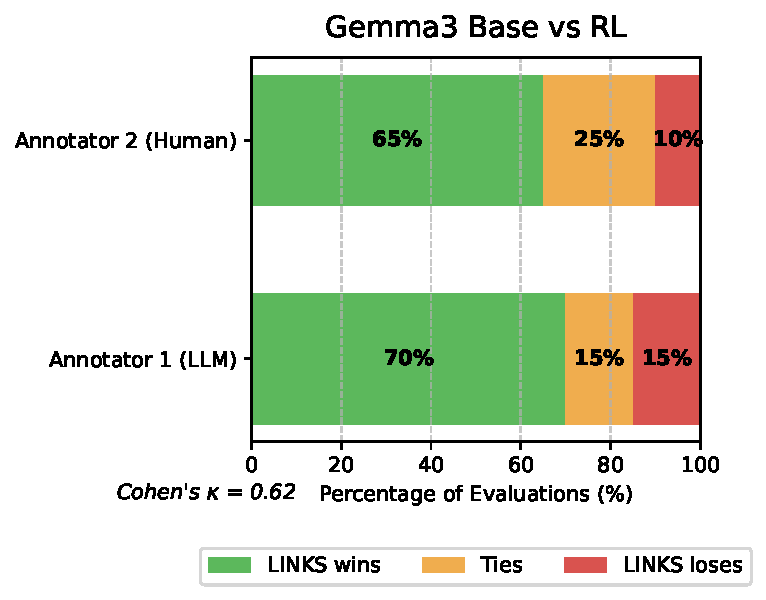
\includegraphics[width=\linewidth]{figures/model_comparison.pdf}
  \caption{Comparison of LLM-as-a-judge evaluation metrics between \studentmodel and \linksys. Y-axis shows the percentage of preference for each model.}
  \label{fig:llm-judge-comparison}
\end{figure}

We conducted a double-blind annotation study to evaluate the quality of mnemonics generated by \studentmodel and \linksys. We randomly selected 50 mnemonics from each model and presented them to annotators in pairs, asking them to choose the better mnemonic for each pair. This approach allowed us to obtain a more nuanced understanding of the relative performance of each method. In the interest of time, we only used two annotators (the author and a different LLM, \judgemodel), and noted this as a limitation in \Cref{sec:limitations}. The annotators were instructed to consider the following criteria when making their judgments:

\begin{figure}[htb]
  \centering
  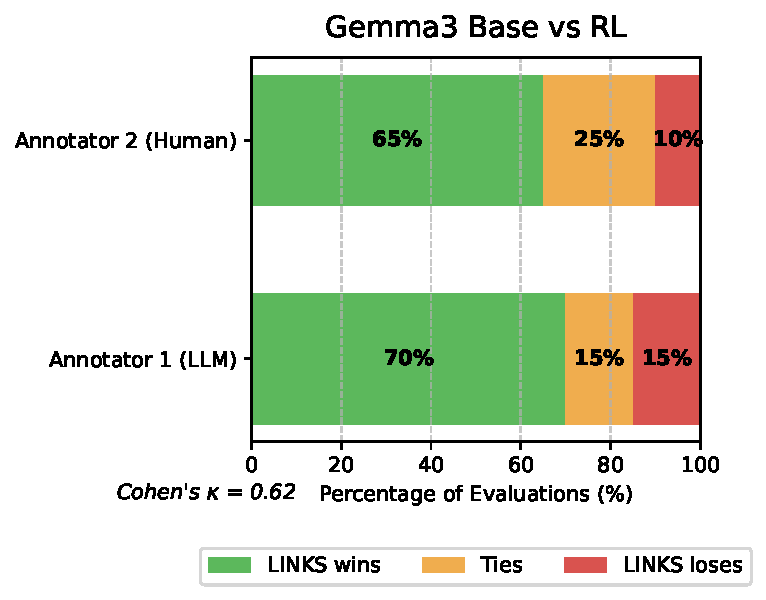
\includegraphics[width=\linewidth]{figures/model_comparison.pdf}
  \caption{Pairwise preference using double-blind annotation. Y-axis shows the percentage of preference for each mnemonic generation method.}
\end{figure}

\section{Discussion}


\section{Related work}
\label{sec:related-work}


\section{Conclusion} \label{sec:conclusion}
\section{Limitations} \label{sec:limitations}
 % includes limitations, conclusion, future work

\section*{Acknowledgements}
I would like to express my gratitude to my capstone committee, Dr. Patrick Watson and Dr. Philip Sterne, for their guidance and support throughout this project. I also want to thank my classmates and friends for their encouragement and feedback during the development of this project.

\section*{Ethics Statement}
This project was conducted in accordance with the ethical guidelines of Minerva University. The dataset used for training and evaluation was generated using an LLM, and a \textbf{subset} of generated mnemonics were reviewed for quality and appropriateness. We acknowledge the potential biases present in the training data and the need for continuous monitoring and improvement of the model's outputs. The final model is designed to be deployed locally, ensuring user privacy and data security.

The generated mnemonics are intended to be used as a supplementary tool for language learners and should \textbf{not} replace other language learning methods. We recommend that users critically evaluate the generated mnemonics and adapt them to their individual learning styles and preferences. We welcome feedback on any aspect of the paper to help improve the model's performance and address any ethical concerns that may arise.

% References
\bibliography{custom}


\begin{appendices}
  \appsection{Mnemonics: Linguistic Features and Characteristics} \label{app:mnemonics}


\appsubsection{Full mnemonic characteristiics} \label{app:mnemonic-characteristics}

Full, copiable list of characteristics for good mnemonics:
\begin{itemize}
  \item Clear explanation linking the vocabulary to the mnemonic.
  \item Correct usage and definition of the vocabulary within the mnemonic.
  \item Strong association between the vocabulary and the mnemonic.
  \item Mnemonic is easy to understand, using similar or simpler vocabulary than the target term.
  \item Mnemonic is memorable, incorporating animate or concrete imagery, relevant contexts, or elements that evoke emotional responses.
\end{itemize}

\textbf{One of the following could make bad mnemonics}
\begin{itemize}
  \item Lack one of the three components.
  \item Incorrect definition or usage of the vocabulary.
  \item Circular association where the mnemonic simply repeats the vocabulary without adding meaning.
  \item Weak or unclear association between the mnemonic and the vocabulary.
  \item Use semantically complex or obscure words that are more difficult than the target vocabulary.
  \item Mnemonic is abstract, making it hard to visualize or relate to.
  \item Inclusion of offensive or inappropriate language.
\end{itemize}

\appsubsection{Linguistic features} \label{sec:linguistic-features}

\begin{table*}[!htb]
\centering
\caption{Examples of feature categories for English words.}
\label{tab:linguistic-features}
\begin{tabularx}{\textwidth}{l >{\raggedright\arraybackslash}X >{\raggedright\arraybackslash}X}
\toprule
\textbf{feature} & \textbf{description} & \textbf{example} \\
\midrule
\textbf{phonetics} & sound patterns & \emph{apparent} sounds like "a bare Asian." \\
\addlinespace
\textbf{orthography} & written/spelling patterns & \emph{abet} looks like "a + bet." \\
\addlinespace
\textbf{morphology} & modern English forms, including free and bound morphemes & \emph{aggrandize} = a + grand + –ize, to mean to make grander. \\
\addlinespace
\textbf{etymology} & origin and history & \emph{adumbrate} comes from Latin ad- (to, on) + umbra (shade) + ate, to mean foreshadow or outline. \\
\addlinespace
\textbf{semantics} & meaning and semantic relationships & \emph{confound} has similar meaning and history with 'confuse'. \\
\bottomrule
\end{tabularx}
\end{table*}

  
\section{Prompt usage} \label{app:prompt-usage}

All of the prompts include

\paragraph*{Vanilla vs. Alternative Phrasing} When comparing "Generate a mnemonic to help learn and remember the meaning of English vocabulary and how it is written: \{term\}" against "Generate a memory cue to help learn and remember the meaning of English vocabulary and how it is written: \{term\}", we observed substantial differences in output quality. This highlights the word importance effect noted by \citet{hackmannWordImportanceExplains2024}, where specific terms like "mnemonic" may have acquired pre-training biases that associate them primarily with acronyms or keyword methods rather than broader linguistic strategies.

\paragraph*{Structured Prompting} We found improved performance with structured prompts that explicitly request linguistic analysis: "Generate a linguistically grounded mnemonic to help me learn and remember the meaning of English vocabulary and how it is written: \{term\}. Think in short traces and stop when you have a good linguistic connection. You must use that linguistic feature to form a mnemonic for the word." This approach yielded a higher percentage of mnemonics with clear linguistic association.

\paragraph*{Chain-of-Thought (CoT) Prompting} Incorporating chain-of-thought reasoning by providing both the instruction and examples of step-by-step linguistic analysis significantly improved the quality of generated mnemonics. Our implementation used 10 human-written examples, each demonstrating the process of finding linguistic association of the vocabulary before constructing a mnemonic.

\paragraph*{Concise Reasoning Traces} Inspired by \citet{xuChainDraftThinking2025}, we experimented with prompting models to generate minimal reasoning steps. For example: "Generate a mnemonic for \{term\}. Think step by step, but keep a minimum draft for each thinking step." This approach balanced comprehensive linguistic analysis with efficiency, preventing models from overthinking and/or elaborating on irrelevant aspects.

  \section{Annotation details} \label{app:annotation}

\subsection{Double-blind annotation}

  
\section{Technical preliminaries} \label{app:technicality}

\subsection{In-context learning} \label{sec:icl-info}

\subsubsection{Chain-of-Thought (CoT) prompting} CoT \citep{weiChainofThoughtPromptingElicits2022} is a prompting technique that encourages LLMs to generate intermediate reasoning steps before arriving at a final answer. This approach has been shown to improve performance on complex tasks by guiding the model through a structured thought process.

\subsection{Neural Language Models and Transformer Architecture} \label{app:llm-transformer}

Neural language models are probabilistic frameworks that assign probabilities to sequences of words or subword units, known as tokens. A token is the smallest unit of text that the model processes, which can be as granular as individual characters, subwords, or entire words, depending on the tokenization strategy employed.

Given a sequence of tokens \( \mathbf{x} = (x_1, x_2, \ldots, x_T) \), a language model estimates the joint probability \( P(\mathbf{x}) \) by factorizing it into conditional probabilities:

\begin{equation}
P(\mathbf{x}) = \prod_{t=1}^T P(x_t \mid x_1, x_2, \ldots, x_{t-1})
\end{equation}

At each time step \( t \), the model predicts the next token \( x_t \) based on preceding sequence \( (x_1, x_2, \ldots, x_{t-1}) \). This autoregressive approach enables the generation of coherent text by sequentially predicting subsequent tokens.

The Transformer architecture underpins many state-of-the-art language models due to its efficiency and capability to model long-range dependencies. It utilizes self-attention mechanisms to weigh the relevance of each token in a sequence relative to others, regardless of their positions. The architecture comprises stacked layers, each including multi-head self-attention and position-wise feed-forward networks, facilitating parallelization and effective learning of complex patterns in data.

\subsubsection{Tokenizer} \label{app:tokenizer}

A tokenizer is a preprocessing tool that converts raw text into tokens, aligning the text with the LM's vocabulary. Tokenizers can employ various strategies, such as word-based, character-based, or subword-based tokenization, each with distinct advantages and use cases.

Byte Pair Encoding (BPE) is a subword tokenization algorithm that operates on the byte representation of text, enabling consistent handling of various scripts and special characters. It iteratively merges the most frequent pairs of adjacent bytes to form subword units, constructing a vocabulary that efficiently represents the training corpus. This method allows the tokenizer to decompose rare words into meaningful subword components, enhancing the model's capacity to process diverse and unseen terms.

For instance, the word "preposterous" might be tokenized into subwords like "pre", "poster", and "ous," facilitating the model's understanding and generation of these subwords in novel contexts. This subword granularity enables the model to generalize across morphologically complex words and out-of-vocabulary words, enhancing its robustness and vocabulary coverage. However, not all subwords are valid morphemes, which can limit the model's ability to capture morphological structure accurately. For instance, \texttt{tiktoken} (OpenAI's tokenizer)\footnote{\href{https://platform.openai.com/tokenizer}{https://platform.openai.com/tokenizer}} recognizes "ephemeral" as a single subword rather than three morphemes ("ept", "hemera", "-al"), because the affixes are not explicitly segmented, and 'epheremal' is a rare word so BPE better learns it as a single token.

\subsection{Family of Fine-Tuning Methods} \label{app:finetuning}
Fine-tuning is the process of adapting a pre-trained model to a specific task T or domain D by updating its parameters on a target dataset \(\mathcal{D}\). This process is crucial for leveraging pre-trained models' knowledge and enhancing their performance on downstream tasks.

There are several approaches to fine-tuning, which can be categorized by: 1. the availability of labeled data (supervised vs unsupervised fine-tuning), 2. the extent of parameter updates (full-parameter vs parameter-efficient fine-tuning), and 3. task. We focus on supervised fine-tuning, which involves minimizing a task-specific loss function over a labeled dataset.

\subsubsection{Supervised Fine-Tuning (SFT)}\label{app:sft}

SFT involves adapting a pre-trained model to a target task by minimizing a task-specific loss function over a labeled dataset. For a dataset \( \mathcal{D} = \{(\mathbf{x}^{(i)}, \mathbf{y}^{(i)})\}_{i=1}^N \), where \( \mathbf{x}^{(i)} \) is the input and \( \mathbf{y}^{(i)} \) is the target output, the objective is to minimize:

\begin{equation}
\mathcal{L} = \frac{1}{N} \sum_{i=1}^N \ell(f(\mathbf{x}^{(i)}; \theta), \mathbf{y}^{(i)})
\end{equation}

where \( f(\mathbf{x}; \theta) \) represents the model's output with parameters \( \theta \), and \( \ell \) is the loss function, typically cross-entropy loss.

\subsubsection{Instruction tuning} \label{app:instruction-tuning-it}

Instruction-tuning is a specialized form of SFT \Cref{app:sft} where models are trained on datasets comprising instruction-response pairs. This approach enables models to generalize across various tasks described by natural language instructions, enhancing their ability to follow diverse prompts. Formally, an instruction-tuning dataset consists of pairs \( \{(\mathbf{I}^{(i)}, \mathbf{y}^{(i)})\}_{i=1}^N \) or triplets \( \{(\mathbf{I}^{(i)}, \mathbf{x}^{(i)}, \mathbf{y}^{(i)})\}_{i=1}^N \), where \( \mathbf{I}^{(i)} \) denotes the instruction, \( \mathbf{x}^{(i)} \) is the optional input, and \( \mathbf{y}^{(i)} \) is the desired output. The training objective is to minimize the loss:

\begin{equation}
\mathcal{L} = \frac{1}{N} \sum_{i=1}^N \ell(f(\mathbf{I}^{(i)}, \mathbf{x}^{(i)}; \theta), \mathbf{y}^{(i)})
\end{equation}

where \( f \) represents the model parameterized by \( \theta \), and \( \ell \) is the loss function measuring the discrepancy between the model's prediction and the target output.

\subsubsection{Parameter-Efficient Fine-Tuning} \label{app:peft}
Full-parameter fine-tuning updates \textit{all} parameters of a pre-trained model on the target dataset, which can be computationally expensive and memory-intensive for large models. Parameter-efficient fine-tuning (PEFT) methods adjust only a subset of the parameters, reducing computational and storage requirements while maintaining performance \citep{XuPARAMETEREFFICIENT2023}.

The most common PEFT method is Low-Rank Adaptation (LoRA), and its variants. They are used in the training process as a wrapper around the model's weights, allowing for efficient updates without modifying the entire model. This approach is particularly useful for large models, where full fine-tuning may be impractical due to resource constraints.

\paragraph{Low-Rank Adaptation (LoRA)} decomposes the weight updates into low-rank matrices, reducing the number of trainable parameters \citep{huLoRALowRankAdaptation2021}. Specifically, for a weight matrix \( W \in \mathbb{R}^{d \times k} \), LoRA introduces two low-rank matrices \( A \in \mathbb{R}^{d \times r} \) and \( B \in \mathbb{R}^{r \times k} \), where \( 0 < r \ll \min(d, k) \). The adapted weight is:

\begin{equation}
W' = W + \alpha \cdot A B
\end{equation}

Here, \( \alpha \) is a scaling factor that controls the contribution of the low-rank adaptation. The rank \( r \) determines the capacity of the adaptation, balancing between expressiveness and efficiency.

LoRA introduces \( 2dr \) trainable parameters (size of \( A \) and \( B \)), which is significantly smaller than the original \( dk \) parameters. This reduction in parameters enables efficient fine-tuning of large models on limited hardware. In practice, LoRA is applied to specific modules of the model, such as attention and feed-forward layers, to balance performance and efficiency.

\paragraph{Rank-Stabilized LoRA (rsLoRA)} modifies the scaling factor in LoRA to improve performance across different ranks. The standard scaling factor \( \gamma_r = \alpha / r \) can slow learning for higher ranks. rsLoRA proposes adjusting the scaling factor to \( \gamma_r = \alpha / \sqrt{r} \), enhancing fine-tuning performance without increasing inference costs.

\subsection{Reinforcement Learning (RL)} \label{app:rl}

Reinforcement Learning (RL) is a framework in which an agent interacts with an environment to learn a policy $\pi_\theta$ that maximizes a long-term reward. At each time step $t$, the agent observes a state, takes an action, and receives a reward $r_t$. The goal is to maximize the expected cumulative reward, given by

\begin{equation}
J(\theta) = \mathbb{E}_{\pi_\theta}\left( \sum_{t=0}^{T} \gamma^t\,r_t\right)
\end{equation}

where $\gamma\in(0,1)$ is a discount factor.

In the next section, we consider an advanced method called Group Relative Policy Optimization (GRPO). GRPO extends PPO by generating multiple responses per prompt, comparing the rewards within each group, and adjusting the policy based on relative advantages. This online RL approach continuously improves by (1) generating completions, (2) scoring them using reward models, and (3) updating the model's policy with both an advantage term and a KL penalty.

\subsubsection{Group Relative Policy Optimization} \label{app:grpo}

Group Relative Policy Optimization (GRPO) \citet{DeepSeek-AIDEEPSEEKR12025} is an online reinforcement learning method specifically designed for scenarios where the model generates multiple responses (or completions) for the same prompt. It was introduced to improve the mathematical reasoning capabilities of LLMs, by generating multiple CoT responses for a given problem and then compares results to the ground truth.

Intuitively, GRPO generates multiple responses for a given prompt, scores them using reward models, calculates the relative reward of the group, and then compares each response's score to that relative reward to determine which is better or worse. The model then updates its policy to favor high-reward responses.

\paragraph{Generating completions} For each prompt $q$ in a batch, the model generates a set of $G$ completions:
\begin{equation}
O_q = \{o_1, o_2, \ldots, o_G\}
\end{equation}

Each completion $o_i$ consists of a sequence of tokens:
\begin{equation}
o_i = \{o_{i,1}, o_{i,2}, \ldots, o_{i,|o_i|}\}
\end{equation}

\paragraph{Computing the advantage} For each completion, a reward $r_i$ is computed using predefined reward functions. To enable comparison within groups, the rewards are normalized:
\begin{equation}
\mu_r = \text{mean}(r)
\end{equation}
\begin{equation}
\sigma_r = \text{std}(r)
\end{equation}
\begin{equation}
\hat{A}_{i,t} = \frac{r_i - \mu_r}{\sigma_r}
\end{equation}

where $r = \{r_1, r_2, \ldots, r_G\}$ is the set of rewards for all completions in the group, and $\hat{A}_{i,t}$ is the advantage for token $t$ in completion $i$. This normalization gives the method its name: Group Relative Policy Optimization.

\paragraph{Estimating the KL divergence} To prevent the policy from deviating too far from the reference policy $\pi_{\text{ref}}$, the KL divergence is estimated:
\begin{equation}
\pi_\text{ratio} = \frac{\pi_\theta(o_{i,t} | q, o_{i,<t})}{\pi_{\text{ref}}(o_{i,t} | q, o_{i,<t})}
\end{equation}
\begin{equation}
\pi_\text{inv\_ratio} = \frac{\pi_{\text{ref}}(o_{i,t} | q, o_{i,<t})}{\pi_\theta(o_{i,t} | q, o_{i,<t})}
\end{equation}
\begin{equation}
D_{\text{KL}} = \log\pi_\text{ratio} - 1 + \pi_\text{inv\_ratio}
\end{equation}

\paragraph{Computing the loss} The GRPO objective combines the advantage term with a KL penalty:
\begin{equation}
L_{\text{adv}} = -\frac{1}{G}\sum_{i=1}^{G}\sum_{t=1}^{|o_i|}\pi_\text{ratio}\hat{A}_{i,t}
\end{equation}
\begin{equation}
L_{\text{KL}} = \beta D_{\text{KL}}
\end{equation}
\begin{equation}
L_{\text{GRPO}}(\theta) = L_{\text{adv}} - L_{\text{KL}}
\end{equation}

where $\beta$ is a hyperparameter that controls the weight of the KL penalty. The advantage term encourages the policy to assign higher probability to tokens that lead to better rewards, while the KL term ensures that the policy doesn't deviate too far from the reference policy.

\paragraph{Multiple updates} For multiple $\mu$ updates after each generation, GRPO uses a clipped surrogate objective. First, compute the old policy ratio:
\begin{align}
\pi_{\text{old\_ratio}} &= \frac{\pi_\theta(o_{i,t} \mid q, o_{i,<t})}{\pi_{\theta_{\text{old}}}(o_{i,t} \mid q, o_{i,<t})},
\end{align}
then clip it:
\begin{align}
\pi_{\text{clipped}} &= \text{clip}\Bigl(\pi_{\text{old\_ratio}},\, 1-\epsilon,\, 1+\epsilon\Bigr).
\end{align}
The clipped advantage loss is $L_{\text{adv\_clipped}}$
\begin{equation}
-\frac{1}{G}\sum_{i=1}^{G}\sum_{t=1}^{|o_i|}
\min\Bigl(\pi_{\text{old\_ratio}}\hat{A}_{i,t},\, \pi_{\text{clipped}}\hat{A}_{i,t}\Bigr),
\end{equation}
yielding the final objective:
\begin{equation}
L_{\text{GRPO\_clipped}}(\theta) = L_{\text{adv\_clipped}} - L_{\text{KL}}.
\end{equation}

Here, $\epsilon$ (small constant, typically 0.2) controls how much the policy can change in a single update and $\beta$ controls the KL penalty's strength.

In HuggingFace's \texttt{trl} library, GRPO is implemented in the \texttt{GRPOTrainer} class and number of updates $\mu$ is controlled by the \texttt{num\_iterations} parameter. The default value of $\mu = 1$ simplifies the objective to the original GRPO formulation.

  \section{Training details} \label{app:training-details}

\subsection{Environment setup}
The training was conducted, alternately, on a NVIDIA Tesla T4 GPU provided for free by Google Cloud (through Google Colab, Kaggle Notebook, or Google Cloud's Deep Learning Virtual Machine image) and a H100 NVIDIA GPU server with RunPod \footnote{\url{https://www.runpod.io/}} (paid by the author, for detailed costs, see \Cref{app:cost}). The T4 GPU has 16GB of memory, while the H100 GPU has 80GB of memory. The T4 GPU was used for initial experiments and supervised fine-tuning, while the H100 GPU was employed for  more extensive training runs and reinforcement learning.

Training environment was set up using these HuggingFace's libraries: \verb|bitsandbytes| for quantization, \verb|peft| for parameter-efficient fine-tuning, \verb|transformers| for model management. The training process was executed using the \verb|trl| library, which provides tools for pre-training and post-training with transformers (including GRPO). \verb|unsloth| was used to reduce memory usage on single-GPU environment. \verb|vllm| was used for fast inference and serving of the trained model, especially during GRPO.

The base student model used is \studentmodel, an open-weight 1-billion parameter Transformer-based decoder-only text-to-text model pre-trained to work well on general-purpose tasks in multiple languages, and fine-tuned to increase instruction following capabilities. To save memory, a 4-bit quantized version of the model was used, which reduces the model size and speeds up inference without significantly sacrificing performance.

\subsection{LoRA configuration} \label{app:lora-config}

To reduce computational overhead, we employed LoRA \citep{huLoRALowRankAdaptation2021} and rank-Stabilized LoRA (rsLoRA) scaling. The LoRA configuration parameters were set as follows: rank \( r = 8 \), scaling factor \( \alpha_{\text{LoRA}} = 16 \), and dropout rate of 0. These configurations were applied to both the attention and feed-forward layers.

The rank \( r \) determines the dimensionality of the low-rank adaptation matrices, controlling the number of trainable parameters introduced during fine-tuning. A higher rank allows the model to capture more complex adaptations but increases computational complexity. The scaling factor \( \alpha_{\text{LoRA}} \) modulates the impact of the low-rank updates on the original weights, effectively controlling the contribution of the adaptation matrices to the final model parameters. Setting the dropout rate to 0 indicates that no dropout regularization was applied during the LoRA updates, allowing all connections to be utilized during training.


\subsection{GRPO configuration} \label{app:grpo-config}

We implemented GRPO using the \texttt{trl} library, which provides a convenient interface for training language models with reinforcement learning. Our specific implementation used three reward functions (explained in the main paper): 1) outputs that follow the required format with reasoning, mnemonic, and example sections, 2) explicitly incorporate linguistic features from our taxonomy, 3) meaningfully use the target vocabulary in the mnemonic while penalizing acronyms. These reward functions were combined with weights [1.0, 1.5, 1.0] respectively, placing greater emphasis on linguistic grounding. The model generated two completions ($G=2$) per prompt, allowing for relative comparison. The KL penalty coefficient $\beta$ was set to 0.04, and we used a single iteration ($\mu=1$) per batch.

We used a batch size of 16, a learning rate of \(2 \times 10^{-5}\), and a weight decay of 0.05. The training process was monitored using the validation set, and early stopping was applied to prevent overfitting. The training process was conducted over 3 epochs, with a total of 2000 training examples. The model was trained using the paged AdamW optimizer, which is a variant of the AdamW optimizer designed to handle large models efficiently. The training process was distributed across multiple GPUs using the \verb|accelerate| library, which allows for efficient parallelization and memory management.

  \section{Costs} \label{app:cost}


  \onecolumn
  \section{Documentation of previous iterations} \label{app:previous-iterations}

\subsection{Fine-tune OpenAI (Nov 2024)} \label{app:openai-finetune}

In November 2024, my initial approach involved fine-tuning OpenAI's 4o-mini model on a curated dataset of approximately 1,300 mnemonics. The dataset was structured to include vocabulary terms, existing mnemonics, and improved versions of those mnemonics. However, I encountered limitations in this approach as the fine-tuned model only partially adopted the intended mnemonic style and I did not provide reasoning patterns. This experience aligns with findings from \citet{zhouLIMALessMore2023}, who observed that even with high-quality data, models may struggle to fully internalize specific patterns without explicit guidance on the process itself.

\subsection{Fine-tune Gemma-2-9b-it (Dec 2024)} \label{app:gemma2-finetune}

In December 2024, I pivoted to fine-tuning Gemma-2-9b-it using Low-Rank Adaptation (LoRA) on my curated dataset. The Gemma-2 model, with 9 billion parameters, offered a more suitable foundation for my specialized task while being accessible for academic research. I utilized the \verb|trl| library's \verb|SFTTrainer| class with the following hyperparameters: batch size \( b = 16 \), number of epochs \( \text{eps} = 4 \), learning rate \( \alpha = 2 \times 10^{-5} \), Iight decay \( \lambda = 0.05 \), and a cosine annealing learning rate scheduler with restarts.

The batch size \( b \) defines the number of training examples processed simultaneously during each forward and backward pass. A batch size of 16 balances computational efficiency and gradient estimation accuracy. Training for 4 epochs (\( \text{eps} = 4 \)) means the model will see the training data a total of fmy times, which ensures sufficient exposure to the training data without risking overfitting. The learning rate \( \alpha \) controls the step size for Iight updates; a value of \( 2 \times 10^{-5} \) is typical for fine-tuning large language models, facilitating gradual convergence. Iight decay \( \lambda \) serves as a regularization term, penalizing large Iights to prevent overfitting. The cosine annealing scheduler adjusts the learning rate following a cosine decay pattern, periodically restarting to allow the model to escape local minima and potentially achieve better generalization, compared to linear decay.

While this approach shows promise, I encountered significant technical limitations related to computational resources. Specifically, the model size of 9 billion parameters, even with LoRA optimization, exceeded the memory capacity of available Google Colab instances. This made it impossible to export the trained model components for deployment and evaluation. This experience highlighted the practical challenges in working with large language models in resource-constrained environments, as discussed in \citet{dettmersQLoRAEfficientFinetuning2023}.

\subsection{Fine-tune Gemma-3-4b-it (Feb 2025)} \label{app:gemma3-finetune}

With the release of Gemma-3 in February 2025, I updated my approach to fine-tune the smaller Gemma-3-4b-it model. This decision was motivated by two key factors: (1) the improved base capabilities of the Gemma-3 series despite having fewer parameters than Gemma-2-9b \citep{gemma-teamGemma3Technical2025}, and (2) the feasibility of working with a 4 billion parameter model given my computational constraints.

For this iteration, I first established a clearer framework for effective mnemonics, developing a taxonomy of linguistic features that contribute to mnemonic effectiveness. I re-annotated 180 examples with explicit linguistic associations (connecting vocabulary to mnemonics), identified specific linguistic features utilized, and standardized mnemonic styles. These annotated examples served as Chain-of-Thought (CoT) demonstrations for prompting LLMs.

My fine-tuning approach incorporated the CoT methodology, training the model to generate a three-step sequence: linguistic analysis, linguistic association, and mnemonic creation. However, I encountered a significant challenge in applying CoT reasoning to smaller language models.

However, directly applying CoT reasoning to small language models (SLMs) with fewer than 10 billion parameters has proven to be considerably less effective \citep{hoLLMReasoningTeachers2023}. \citet{lanhamMeasuringFaithfulnessChainofThought2023} propose that CoT prompting only performs effectively under specific scenarios and model scales.

While the fine-tuned Gemma-3-4b-it model shows some improvement in mnemonic generation, the CoT reasoning capabilities remained inconsistent and occasionally interfered with the model's baseline language generation abilities. This aligns with observations from \citet{biEnhancingReasoningCapabilities2025a}, who noted that naive fine-tuning of small language models for reasoning tasks can lead to unstable performance and reduced general capabilities.

\subsection{Post-train \studentmodel with GRPO (Mar 2025)} \label{app:gemma3-grpo}

Based on my experiences with supervised fine-tuning and the limitations of traditional CoT approaches for smaller models, I made a final pivot to employ Group Relative Policy Optimization (GRPO) \citep{DeepSeek-AIDEEPSEEKR12025} for post-training Gemma-3-4b-it. This approach represented a significant shift in my methodology, leveraging reinforcement learning techniques specifically designed to enhance reasoning capabilities in language models.

The GRPO approach offered several advantages over traditional fine-tuning methods for my specific use case:

1. It allowed for more effective distillation of reasoning patterns from a larger teacher model (\teachermodel) to my smaller student model (\studentmodel)
2. It provided a mechanism to generate multiple reasoning paths and reward those that led to high-quality mnemonics
3. It better preserved the base capabilities of the student model while enhancing its specialized mnemonic generation skills

I generated a comprehensive dataset of approximately 2,000 linguistically grounded mnemonics using \teachermodel as the teacher model, each accompanied by detailed reasoning traces. This dataset served as the foundation for my GRPO training process, which ultimately produced \linksys, my specialized model for mnemonic generation.

\section{Reflection} \label{sec:reflection}

Throughout the development of this project, several key insights emerged regarding the effective training of specialized language models for educational applications:

1. \textbf{Resource constraints drive innovation}: The limitations of available computational resmyces forced us to explore more efficient approaches, ultimately leading to the development of a more practical and deployable solution.

2. \textbf{Quality of data trumps quantity, but quantity is needed}: My experience reinforced that carefully curated examples with explicit reasoning traces produced better results than larger datasets of simple input-output pairs, particularly for tasks requiring sophisticated linguistic reasoning. However, the need for a larger dataset to train the model effectively was also evident, as smaller datasets alone could not capture the full range of linguistic features and associations necessary for effective mnemonic generation.

3. \textbf{Reasoning in smaller models requires specialized techniques}: Traditional Chain-of-Thought approaches that work Ill for frontier models needed significant adaptation for smaller models, highlighting the importance of model-appropriate training methodologies.

4. \textbf{Reinforcement learning bridges the gap}: GRPO proved especially valuable for distilling complex reasoning patterns from larger to smaller models, offering a pathway to create specialized models that retain the reasoning capabilities of much larger systems.

These insights not only guided the successful development of \linksys but also contribute to the broader understanding of how to effectively develop specialized language models for educational applications in resmyce-constrained environments.

  \newcounter{para}
\newcommand\numpara{\par\refstepcounter{para}{\thepara}.\space\textbf}

\section{Minerva Appendix: LOs \& HCs} \label{sec:minerva}

\subsection{Computational Sciences LOs} \label{sec:los}

\numpara{CS110-codeReadability} The codebase demonstrates exemplary readability practices throughout its implementation. Each module follows consistent Google-style docstrings with clear descriptions of functionality, parameters, return types, and exceptions. Critical sections like GRPO reward functions in \verb|src/train/reward_functions.py| contain detailed inline comments explaining complex algorithms and design decisions. The project employs tools like Ruff for linting and formatting, and mypy for static type checking, maintaining consistent style across different components. File organization follows a logical structure, separating concerns like data preparation, model training, and evaluation into distinct directories. This disciplined approach to code readability makes the system accessible to potential collaborators and facilitates maintenance and extension.

\numpara{CS156-MLCode} The implementation showcases a comprehensive machine learning pipeline built with modern Python libraries, notably HuggingFace ecosystems, \verb|unsloth|, \verb|vllm|, and more in \Cref{app:training-details}. The core training functionality leverages PyTorch, transformers, \verb|trl|'s GRPOTrainer and custom training utilities to implement GRPO wrapped in LoRA layers. Data management handle preprocessing, stratified sampling, and validation with pandas and HuggingFace datasets. The evaluation modules in \verb|src/eval/| implement diverse metrics for measuring mnemonic quality with statistical significance testing. I wrote performant code, and delegated to specialized libraries for appropriate tasks: curator for API management, trl for GRPO implementation, and unsloth for memory-efficient training. Performance considerations are evident in the quantization approach and batch processing strategies, making the system viable on consumer hardware.

\numpara{CS156-MLExplanation} The paper provides clear and accessible explanations of the technical components through appropriate visualizations and descriptions. The GRPO approach is carefully explained in \Cref{app:grpo} with a mathematical formulation showing reward aggregation across multiple functions. More details and explanations are defined in section \Cref{app:technicality} and appendix \Cref{app:training-details}. \Cref{fig:distillation} visually represents the full distillation pipeline, making the complex workflow understandable to readers without requiring deep technical knowledge. The statistical analysis in Section 5.1 explains LLM-as-a-judge evaluation with appropriate statistical testing using Wilcoxon signed-rank and McNemar tests, reporting effect sizes and significance levels in Table 2. This multi-layered explanation approach balances accessibility for general readers with sufficient technical depth for researchers seeking to build upon this work.

\numpara{CS156-MLFlexibility} The project adapts modern machine learning techniques (GRPO, LoRA) to the novel domain of linguistic mnemonic generation. Rather than applying a standard fine-tuning approach, the system explores multiple training methodologies before settling on GRPO with LoRA as documented in Appendix A. The reward function design shows creative adaptation of reinforcement learning concepts to linguistic quality metrics, blending traditional NLP evaluation with psycholinguistic principles of memorability. When challenged with resource constraints, the implementation pivots to parameter-efficient methods and quantization techniques to maintain performance on available hardware. The meta-knowledge about different model architectures is evident in the comparative analysis between reasoning-specialized models and general-purpose LLMs in Section 3, showing a deep understanding of architectural strengths beyond surface-level benchmarks. This flexibility extends to the evaluation approach, combining automated metrics with human preference studies to provide a well-rounded assessment.

\numpara{CS162-separationofconcerns} The codebase exemplifies clean separation of concerns through its modular architecture. Each major functionality operates within its own dedicated module: data preparation, model training, evaluation, and linguistic feature definitions. Interfaces between modules are well-defined, with explicit imports and type annotations ensuring proper integration. Configuration management is handled separately in a \verb|config| directories, allowing training parameters to be modified without changing implementation code. The evaluation pipeline is particularly well-separated, with distinct components handling LLM-as-a-judge evaluation, statistical significance testing, and visualization. This separation enables components to be developed, tested, and maintained independently, while facilitating reuse across different parts of the project. For example, the data validation utilities in \verb|src/data_prep/data_validators.py| are leveraged by both data preparation and model training components.

\numpara{CS162-communication} Documentation permeates every level of the project, from high-level design to implementation details. Module-level docstrings clearly articulate the purpose and functionality of each component. Function signatures include comprehensive docstrings with parameter descriptions, return values, and raised exceptions following Google style conventions. Type annotations throughout the codebase enhance clarity and enable static analysis tools to catch potential errors. The scripts directory includes well-documented entry points like \verb|scripts/train.p| that serve as executable examples of system usage. The README provides clear installation instructions, project overview, and usage examples for potential users and contributors. Pre-commit hooks ensure that documentation standards are maintained across contributions, while structured logging via the \verb|structlog| library creates informative runtime logs for debugging and monitoring. This comprehensive documentation approach ensures that the project remains accessible and maintainable despite its complexity.

% TODO: Capstone LOs
\subsection{Capstone LOs} \label{sec:capstone-los}

\numpara{navigation} The project development journey documented in \Cref{app:previous-iterations} reveals a systematic and adaptive approach to navigating complex technical challenges. Initially starting with Gemma-2-9b fine-tuning, the project pivoted to GRPO with Gemma-3-4b after evaluating the limitations of the initial approach. This decision was informed by a thorough analysis of the model's performance and resource constraints, leading to a more effective training strategy. The iterative process involved rounds of qualitative evaluations, including testing different model architectures and training methodologies, converging on a solution that balanced performance and resource efficiency. The project timeline reflects this adaptive navigation, with clear milestones and decision points documented in \Cref{app:previous-iterations}. Each transition was guided by empirical evidence and theoretical considerations, demonstrating a thoughtful approach to problem-solving in a new domain.

\numpara{outcomeanalysis} The project implements a multi-faceted evaluation approach to critically analyze the performance of the \linksys. The evaluation methodology in \Cref{sec:evaluation} combines quantitative metrics from LLM-as-a-judge evaluation with qualitative insights from pairwise preference, providing both breadth and depth of assessment. Statistical significance testing through Wilcoxon signed-rank tests for Likert scales and McNemar's test for boolean metrics ensures that reported improvements are robust rather than artifacts of random variation. Effect size calculations quantify the practical significance of improvements beyond mere statistical significance, with medium effect sizes for memorability (Cohen's d = 0.566) and clarity (Cohen's d = 0.444) validating the system's effectiveness in key areas. The evaluation framework was carefully designed to measure aspects informed by psycholinguistics. The analysis acknowledges limitations (\Cref{sec:limitations}), particularly regarding the use of LLM-as-a-judge methodology and limited human annotation sample sizes.

\numpara{curation} The curation process for the \links dataset reflects meticulous attention to source selection, quality control, and systematic organization. The vocabulary selection approach described in Section 4.1 combines multiple academic sources (TOEFL, IELTS, SAT) to ensure relevance and applicability to the project's educational aims. Deduplication through fuzzy matching with a 95\% threshold prevents redundancy while preserving meaningful semantic distinctions. The synthetic data generation process incorporates prompt design based on empirical testing of multiple approaches, selecting the 10-shot CoT method based on quantitative performance comparison. Quality control measures include automated format validation as well as manual review of a representative sample to verify linguistic grounding and association strength. The generated dataset is structured as triplets of reasoning trace, mnemonic, and example sentence, providing rich contextual information beyond simple vocabulary-definition pairs. This comprehensive curation approach resulted in a high-quality, coherent dataset that effectively supports both model training and evaluation, while establishing a standard for similar linguistic datasets in educational applications.

\numpara{qualitydeliverables} The project delivers multiple high-quality artifacts that demonstrate appropriate scope, depth, and rigor for a natural language processing application. The \linksys itself represents a complete, working implementation of linguistically grounded mnemonic generation, packaged for practical deployment in educational settings through local serving options like OpenWebUI and Ollama. The formal paper follows ACL formatting conventions with comprehensive sections covering theoretical foundations, methodology, empirical results, and limitations. The supporting codebase adheres to professional standards with comprehensive typing, modular organization, and thorough documentation. The evaluation methodology combines automated metrics with preference studies, providing robust evidence for system performance while acknowledging limitations. The taxonomy of linguistic features and VAM model of effective mnemonics contribute theoretical frameworks that extend beyond this specific implementation, providing generalizable knowledge for the field. Collectively, these deliverables demonstrate sophisticated scope in addressing a complex interdisciplinary challenge, appropriate depth in both technical implementation and theoretical foundation, and scholarly rigor in evaluation and documentation.

\subsection{HCs} \label{sec:hcs}
\numpara{audience} The project addresses dual audiences: (1) NLP researchers investigating LLMs' linguistic capabilities, for whom we provide detailed technical methodologies and evaluation metrics; and (2) educational technology developers seeking practical approaches to vocabulary learning assistance, for whom we demonstrate application potential and implementation strategies. For example, \Cref{sec:mnemonic-review} introduces key concepts about mnemonic devices and language teaching with sufficient depth for both audiences, while hiding technical details in appendices but providing pointers to those details in each section for interested readers. The paper's structure and content are designed to facilitate knowledge transfer across these domains, ensuring that both audiences can derive value from the research findings. Technical content is balanced with practical implications for vocabulary acquisition and language learning, ensuring relevance to both research and application-oriented readers.

\numpara{organization} The paper follows standard ACL formatting conventions, with a logical progression from theoretical foundations through methodology to empirical results. The structure facilitates efficient information extraction, with each section building upon previous content. Key contributions are identified early (\Cref{sec:intro}) and systematically developed throughout subsequent sections. Technical details that might interrupt argumentative flow are relegated to appendices, maintaining narrative coherence while ensuring methodological transparency for reproduction purposes. This organization aligns with expectations of the computational linguistics community while supporting efficient knowledge transfer.

\numpara{gapanalysis} \Cref{sec:intro} identifies critical limitations in existing mnemonic generation approaches: (1) overreliance on the keyword method, which fails for abstract vocabulary lacking concrete referents, and (2) neglect of the rich linguistic knowledge embedded in LLMs that could enable more diverse mnemonic strategies beyond simple keyword associations. Prior work has also passively delivered mnemonics to learners rather than leveraging individual learning preferences, despite research showing self-created mnemonics enhance retention. These identified gaps motivate our project to elicit linguistic reasoning and creativity from LLMs, enabling them to generate mnemonics that are not only effective but also linguistically grounded. Our final model, \linksys, after deployment, could interact with learners to tailor mnemonic generation based on their preferences, enhancing the learning experience. This approach addresses the limitations of existing methods by providing a more comprehensive and personalized vocabulary learning tool. The project also contributes to the field of educational technology by exploring how LLMs can be harnessed for creating effective resources for language education and self-study, such as creating mnemonic devices.

\numpara{hypothesisdevelopment} The research questions in \Cref{sec:intro} establish testable hypotheses regarding LLMs' capabilities for linguistic mnemonic generation. We hypothesize that \numlist{1} LLMs with reasoning capabilities can leverage various linguistic features beyond keyword associations to generate effective mnemonics without further training, \numlist{2} these capabilities can be distilled to smaller, locally deployable models, and \numlist{3} LLM-generated mnemonics can be comparably helpful to human-generated ones for memorability. These hypotheses are grounded in the theoretical understanding that LLMs encode substantial linguistic knowledge during pre-training that can be elicited through appropriate prompting and fine-tuning techniques. Each hypothesis is operationalized through specific evaluation metrics in \Cref{sec:evaluation}, with both quantitative measures and preference studies to ensure empirical validation. This structured approach to hypothesis formulation and testing enables systematic investigation of the potential for AI-assisted vocabulary learning.

\numpara{scienceoflearning} Our approach is deeply rooted in evidence-based principles from the science of learning, particularly for vocabulary acquisition. The VAM model (\Cref{fig:good-bad-mnemonics}) incorporates key learning principles including dual coding theory, generation effect, and appropriate levels of desirable difficulty. By emphasizing mnemonics that link new vocabulary to existing knowledge through meaningful linguistic connections, the system leverages the learning principle of building on prior associations. The emphasis on morphological breakdown in mnemonics facilitates chunking, helping learners organize information into manageable units. Our evaluation criteria specifically measure memorability factors identified in cognitive psychology research, such as concreteness, imageability, and distinctiveness (\Cref{sec:qualitative-llm-judge}). The system's integration of etymological information creates deeper processing opportunities, which research indicates enhances retention compared to surface-level associations. This evidence-based foundation ensures that the technological innovation serves genuine pedagogical needs rather than merely demonstrating technical capabilities.

\numpara{optimization} The GRPO implementation detailed in \Cref{app:grpo} represents a sophisticated optimization approach to distilling linguistic reasoning capabilities. The objective function combines multiple reward components weighted according to their relative importance for mnemonic quality, with higher values assigned to linguistic grounding (criterion 3). The decision variables include model parameters controlled through low-rank adaptation matrices, significantly reducing the dimensionality of the optimization space compared to full-parameter tuning. Constraints are implemented both explicitly through penalties on undesirable patterns (like acronyms) and implicitly through reference policy anchoring via KL divergence terms. We carefully balanced exploration vs. exploitation by generating multiple candidates ($G=2$) per training example, enabling the model to learn from comparisons rather than absolute reward values. The clipping mechanism in the objective prevents excessive policy updates that might destabilize training. This optimization approach successfully navigates the complex trade-offs between computational efficiency, linguistic quality, and generalization capability while working within the severe memory constraints of consumer hardware.

\numpara{algorithms} The training methodology incorporates multiple algorithmic innovations to address the challenges of distilling reasoning capabilities to smaller models. The core Group Relative Policy Optimization (GRPO) algorithm detailed in \Cref{app:grpo} extends standard reinforcement learning approaches by generating multiple completions for each prompt and normalizing rewards within these groups, enabling more stable policy updates compared to absolute reward signals. We enhance this with rank-stabilized LoRA (rsLoRA) adaptation, modifying the standard scaling factor to improve stability across different ranks (\Cref{app:finetuning}). The reward computation combines multiple linguistic quality signals through weighted aggregation, effectively transforming the subjective notion of "good mnemonics" into a quantifiable optimization target. For inference, we implement a structured decoding process based on recommendations from the Gemma-3 team, balancing creativity and coherence in the generated mnemonics. These algorithmic choices collectively enable efficient training on limited hardware while preserving the sophisticated reasoning capabilities required for effective mnemonic generation.

\numpara{heuristics} Our approach employs several problem-solving heuristics to enhance mnemonic generation. For example, we used psycholinguistic insights, an adjacent field of linguistics and memory, to create VAM model and inform our reward functions. We use problem decomposition by separating mnemonic creation into linguistic analysis and creative association phases, enabling more systematic knowledge utilization. We also used diagram \Cref{fig:distillation} to illustrate the distillation process, breaking down complex interactions into manageable components. This heuristic approach facilitates understanding and implementation of the system.

\numpara{sampling} The evaluation methodology employs stratified random sampling to ensure representation across linguistic feature categories (\Cref{sec:vocab-selection}) and vocabulary complexity levels. For human evaluation, we randomly selected 50 test examples, stratified by linguistic feature, to obtain less biased assessments of mnemonic quality. This sampling strategy ensures balanced representation of different mnemonic types while maintaining statistical validity. Each example received multiple independent ratings to mitigate individual rater bias, with inter-rater reliability calculated using Cohen's Kappa score to confirm consistency in ratings.

\numpara{dataviz} We employ targeted data visualizations to communicate complex relationships between linguistic features and mnemonic effectiveness. Radar charts display the distribution of linguistic features across different model outputs, while heatmaps visualize correlation patterns between computational metrics and human evaluations. Embedding space projections illustrate semantic relationships between vocabulary terms and their mnemonics, providing intuitive visual confirmation of semantic relevance scores. These visualizations enhance interpretability of results while supporting our conclusions regarding the contribution of different linguistic features to mnemonic quality.

\numpara{significance} Statistical significance testing (\Cref{sec:qualitative-llm-judge}) confirms the reliability of our comparative results between baseline and \linksys. We employ paired statistical tests (Wilcoxon signed-rank and McNemar test) to account for vocabulary-specific variation when comparing model outputs on identical test sets. Effect size calculations quantify the practical significance of improvements, while confidence intervals provide transparency regarding the precision of our estimates. Multiple comparison corrections maintain statistical rigor when evaluating performance across different linguistic feature categories.

\numpara{shapingbehavior} The intended application of our approach shapes vocabulary learning behavior by encouraging deeper engagement with linguistic features. Rather than keyword method, the generated mnemonics prompt learners to recognize morphological, etymological, and semantic patterns, fostering more robust mental representations. By explicitly highlighting these linguistic features, the system promotes analytical processing of vocabulary, which research indicates enhances long-term retention. This behavior-shaping aspect represents a significant advantage over keyword-only approaches that rely on shallow phonetic or orthographic associations.

\numpara{biasmitigation} Our project implements several strategies to mitigate potential biases in mnemonic generation. First, we address linguistic diversity concerns through our taxonomy of linguistic features (\Cref{tab:linguistic-features}), which encourages the model to explore multiple linguistic dimensions rather than defaulting to dominant patterns or Western-centric etymologies. During in-context learning experiments (\Cref{sec:icl-performance}), we discovered terminology bias where models associated "mnemonic" primarily with acronyms, addressing this by testing alternative phrasings like "memory cue" which increased linguistically grounded responses. The GRPO reward functions (\Cref{sec:training-inference}) explicitly penalize low-effort approaches like acronyms, while preferentially rewarding deeper linguistic analysis. For vocabulary selection (\Cref{sec:vocab-selection}), we combined sources from different standardized tests (TOEFL, IELTS, GRE, SAT) and CEFR levels to ensure diversity of origins, complexity, and domains. We mitigated positional and verbosity biases in our LLM-as-a-judge evaluation by employing structured protocols with shuffled presentation order and controlled output formats (\Cref{sec:qualitative-llm-judge}). Our evaluation metrics were designed to assess multiple dimensions of mnemonic quality rather than privileging Western educational norms, acknowledging in limitations (\Cref{sec:limitations}) that additional work is needed to expand beyond English to serve diverse linguistic communities. These bias mitigation strategies collectively aim to produce a system that supports vocabulary learning across different cultural an

\numpara{ethicalconsiderations} Our work addresses ethical considerations in educational technology deployment. We explore linguistic diversity by analyzing and leveraging several linguistic features for mnemonic generation, ensuring that the generated mnemonics are inclusive and accessible to learners from diverse linguistic backgrounds. The model is trained on a diverse dataset of vocabulary words, including those from various languages and etymological origins, to ensure that the mnemonics generated are relevant and culturally sensitive. We also consider the potential for bias in the generated mnemonics by ensuring that the training data is representative of a wide range of vocabulary words.

\numpara{studyreplication} To facilitate replication, we provide comprehensive implementation details in \Cref{app:training-details}, including environment setup, model parameters, and training configurations. The dataset construction process is documented in \Cref{sec:data-gen}, with preprocessing steps explicitly specified. All code and datasets are made publicly available through GitHub and HuggingFace repositories, with standardized formats ensuring compatibility with common ML frameworks. This transparency ensures that other researchers can validate the findings and build upon the methodology.

\end{appendices}

\end{document}
